\documentclass[12pt]{report}
\usepackage[T1]{fontenc}
\usepackage[utf8]{inputenc}
\usepackage{graphicx}
\usepackage{amsmath,amssymb,amsfonts}
\usepackage{txfonts}
\usepackage{url}

%\usepackage[polish]{babel}

\renewcommand{\chaptername}{Chapter}
\renewcommand{\contentsname}{Table of contents}
\renewcommand{\figurename}{Fig.}
\renewcommand{\tablename}{Tab.}
\renewcommand{\listfigurename}{List of figures}
\renewcommand{\listtablename}{List of tables}
\renewcommand{\bibname}{Bibliography}

\pagestyle{headings}

\setlength{\textwidth}{14cm}
\setlength{\textheight}{20cm}

\newtheorem{definition}{Definition} % przykład nowego środowiska 
\newtheorem{example}{Example}[chapter] % przykład nowego środowiska 
\newtheorem{corollary}{Corollary}[chapter] % przykład nowego środowiska [corollary => wniosek] 



\begin{document}
\tableofcontents	% generuje spis treści ze stronami !!!

%\indent - wymuszony odstep
%\bf - pogrubienie

\chapter{Introduction} \label{rozdz.wstep} 
In the age of ubiquitous Internet access more and more human activities take place in the Web. E-commerce, the act of shopping online, has been on the increase for many years. [{\bf tutaj jakies statystyki, dane nt udzialu ecommerce w ogolnej sprzedazy}]

The amount of products offered on the Internet can be overwhelming for an average consumer, therefore companies take efforts to properly target users with relevant content. Correct product targeting directly translates to increased sales. [{\bf jakis reference}] Systems responsible for this are {\bf recommender systems}.

In the last several years the world has witnessed the rise of social media - Internet-based applications enabling users to connect with each other and share various content. The principal services include Facebook, Twitter and LinkedIn. This phenomenon enabled large-scale user information gathering. That information can be shared with third parties (with user consent) and can be used by them to improve user experience. [{\bf doszlifowac}]

The use of social media in e-commerce is commonly referred to as {\bf social commerce}. According to Lora Cecere of Altimeter Group \cite{rise_of_social_commerce}, "Social Commerce is the use of Social Technologies to connect, listen, understand and engage to improve the shopping experience."

% The aim of this thesis is to create a recommender system that leverages user social media information to suggest products. The implementation will be a demo web e-commerce store.[{\bf rozwinac?}]


% Tutaj ogólnie w skrócie o wzroście znaczenia ecommerce, social commerce etc.
% Coraj więcej produktów, czasem trudno się w tym odnaleźć.
% Rekomendacje dobre zarówno dla klientów (szybciej mogą znaleźć to, czego potrzebują), jak i dla sklepów (większe zyski).

\section{Scope of work}
The thesis involves the areas of software engineering, web development, systems integration and recommender systems.

The aim of this thesis is to design and create a recommender system that leverages users' social media information to suggest products. 

While there exist many recommender systems, most of them require initial information about user preferences regarding some part of data that the later recommended items come from. For example, if a user is to be recommended a movie to watch, the system needs either a history of movies the user has seen, his ratings on multiple movies etc. [{\bf dopracowac}] Next, this information can be processed in two ways:
\begin{itemize}
\item collaborative filtering - based on item ratings, other users with similar tastes are found and items they like are proposed
\item content-based filtering - based on item ratings, items similar to the highest ranked items are found and proposed
\end{itemize}



Są już systemy rekomendacyjne, ale cierpią na 2 główne problemy: cold start i data sparsity. 
Wykorzystanie grafowej bazy danych, dobrze modelującej relacje społeczne.

Osoba podejmująca tematykę stoi przed wyzwaniami: zbudować rzetelną bazę produktów, bazę użytkowników, przekonać użytkowników do udostępnienia danych osobowych etc.

Spodziewane efekty:\\
- rzetelne rekomendacje tuż po zalogowaniu użytkownika\\
- ...\\

% Dlaczego podejmowanie tej tematyki jest potrzebne? Czy są inne
% rozwiązania tego problemu/tych problemów? Jakie? czy są lepsze/gorsze,
% tańsze/droższe, itp.
% \indent Przed jakimi wyzwaniami stoi osoba podejmująca tematykę? \\
% \indent {\bf Określić spodziewane efekty pracy:} W wyniku doświadczeń przeprowadzonych w zakresie pracy polepszeniu
% uległo.... podać konkretne wskaźniki rezultaty, jak np. przyspieszenie obliczeń,
% redukcja kosztu, nowe oprogramowanie itp. w złotówkach, sekundach, procentach,
% roboczogodzinach itp. 

% {\bf (razem max. 3 strony - strona przeliczeniowa = 1800 znaków, średnio 30
% wierszy po 60 znaków)}

\section{Objectives}
Wymienić w punktach cele pracy, rozpoczynając od celów poznawczych (dotyczą\-cych
zebrania wiadomości, przybliżenia/popularyzacji technik / metod / zagaadnień).
W~drugiej kolejności wyienić cele praktyczne.
\subsubsection{Przybliżenie (popularyzacja) metody/technologii/systemu...}
\subsubsection{Propozycja rozwiązania problemu....}
\subsubsection{Opis zastosowania technologii X w problemie Y...}
\subsubsection{Przedstawienie prototypu systemu/układu/aplikacji...}
\subsubsection{Określenie przydatności algorytmu Z do rozwiązania problemu T.....
}
\subsubsection{Opracowanie strategii ... w celu poprawy wydajności/jakości...}
\subsubsection{Ocena możliwości wdrożenia proponowanych rozwiązań, ich wartość
praktyczna, lokalne i globalne możliwości zastosowania}
\subsubsection{itp.}

Każdy cel opisać w minimum 2-3 zdaniach. Użyte określenia muszą być powszechnie
zrozumiałe, nie stosujemy skrótów, slangu,  tzw. makaronizmów, np. ,,softłer''.
{\bf cały podrozdział ok. 1 strony przeliczeniowej czyli 1800 znaków}

\section{Research method}
\begin{itemize}
\item Studia literaturowe
\item Analiza budowy i działania istniejących produktów
\item Projektowanie i prototypowanie nowatorskich rozwiązań 
\item Obliczenia i ........
\end{itemize}

Każdy element opisać w minimum 2-3 zdaniach. Np. studia literaturowe powinny
odnosić się do charakterystyki wykorzystanych źródeł książkowych, czyli: Jaka
jest podstawowa literatura dziedziny, czy jest dostępna w języku polskim, czy trzeba je tłumaczyć, czy wiedza na ten
temat jest zebrana w jednym miejscu, czy jej synteza jest osobnym zadaniem itp. 
Jak duży jest udział źródeł elektronicznych w tej ,,działce'' wiedzy i badań,
itd. \\
\indent Jakie metody badawcze są typowe dla danego tematu. Dlaczego je
zastosowano, ewentualnie dlaczego zastosowano inne? \\
WYMAGANE ODNOŚNIKI DO POZYCJI BILIOGRAFII.\\
{\bf cały podrozdział ok. 1 strony przeliczeniowej czyli 1800 znaków}.

\section{Literature overview} % ?? czy to będzie ?
Rozszerzyć odpowiedni podpunkt z metody badawczej, np. wg podziału:
\subsubsection{Źródła książkowe polskojęzyczne i tłumaczenia}
\subsubsection{Źródła książkowe obcojęzyczne}
\subsubsection{Artykuły naukowe, raporty z badań, komunikaty konferencyjne,
dokumentacje techniczne, manuale, instrukcje}
\subsubsection{Źródła elektroniczne}


\section{Thesis plan}
Tematem pracy jest: ....., zaś za główny cel przyjęto ...... . \\
Rozdział \label{rozdz.wstep} zawiera wstęp i cele pracy. W rozdziale drugim
opisano/...... w Rozdziale 3. zawarto............ Rozdział 4. przedstawia..... \\
W podsumowaniu pracy przedstawiono..........................., z czego wynika,
że ................  \\
Najważniejszym wnioskiem/wynikiem/rezultatem pracy jest..................\\ {\bf wyraźnie określić
CO TO JEST}. \\

{\bf cały podrozdział ok. 1 strony}.




\chapter[Fundamental information on social...]{Fundamental information on social commerce and recommendation algorithms} \label{fundamental_info}


% \section{Podstawowe definicje}
% Ten podrozdział powinien zawierać dokładny opis terminologii  pojęć zasadniczych dla tematu pracy, którymi autor będzie się posługiwał przy realizacji głównych celów pracy. 


% \section{Istniejące rozwiązania w dziedzinie}
% W tym podrozdziale zostaną opisane.....
% \subsection{Sprzęt}
% .........................
% \subsection{Oprogramowanie i wdrożone systemy}
% .....................................
% \subsection{}
% ...................

% \section{Wady i słabe punkty istniejących rozwiązań}
% \subsection{Efektywność}
% ..........................
% \subsection{Utrudniony dostęp}
% ..............
% \subsection{Wysokie koszty}
% ...............................



\chapter{Presentation of existing recommender systems}

\section{A Social Network-Based Recommender System (SNRS)}


% % %
\chapter{Implementation of new functionalities}

\section{Overview}
\subsection{General idea}
In order to implement and test the system I have decided to build a web application. It is a sample e-commerce store that will gather information about users from their social network. Additionally it will contain a list of exemplary products from different categories, which will be recommendable items. 

The general idea was to implement the so-called "social login" - \cite{social_login} a feature enabling the user to log in to a third-party website using existing login information from a social networking service, without the need of creating a new login account specifically for that website. A website using this feature can request additional information from the user's profile, such as gender, location, list of friends, interests etc. 

Thanks to this, a newly logged user would not be anonymous for my application. By requesting appropriate information from the social network I would be able to analyze user's data and compare them to other existing users in my database. As a result, it would be possible to calculate similarities between users, which is a crucial step in recommender systems.

It is worth noting that the user similarity computation would occur before any interaction of the user with my application. This is a major difference as opposed to classical collaborative filtering approaches, where in order to find nearest neighbours (most similar users) users are compared in terms of their preferences towards recommendable items (e.g. ratings of movies). In my case only the information derived from social networks influences the similarity.

As a consequence, the new approach enables serving recommendations to new users right after their login to the website. The only limiting factor is data downloading from the social network and computation time. Nevertheless, it is safe to assume that the result could be presented withing tens of seconds after the login step. Even if it is not instantaneous, in a typical use case the time needed for recommendation computation would allow the user to get familiar with the website's layout, functionalities etc. When the results would be ready, they could be asynchronously loaded onto the page. 

The only prerequisite for such a situation is that there exists a reasonable user base of the service. Moreover, the system needs to both possess the users' social network information and to know their preferences towards the system's items. Therefore, in a typical scenario of implementation in an existing service, first the social login and social information acquisition would be enabled. After a period of gathering the preferences of socially-logged users, via their item ratings, shopping/browsing history, comment analysis etc., the initial user base would be established. In the second phase, each new user could obtain recommendations. Obviously, the system will improve over time, as more and more users with social data and product preferences are in the database.

\subsection{Solution plan \textit{[?]}}

The system implementation will be conducted in two stages.
\begin{enumerate}
\item Users will be able to log in to the website with their social network account. Next, they will be asked to complete a survey, in which they will rate products in the store's catalog according to their tastes. No recommendation will be offered at this point.
\item Having the initial user base, any new user logging in with the social network will be presented with instant recommendations on products.
\end{enumerate}

The social network that the application will integrate with is Facebook. After research it was found that Facebook can provide most useful user information. Moreover, it is the most popular social network in Poland, therefore it will be easiest to find volunteers eager to provide their data to the project.

\subsection{Technologies}
\subsubsection{Web application}
The main development language is Java 8. The web application is created using Spring Framework 4 \cite{spring_framework}, with Spring MVC as the model-view-controller design pattern implementation and Thymeleaf as the template engine. 

The front-end of the website uses the typical web technology stack: HTML / CSS / JavaScript (jQuery). A free theme for the Bootstrap front-end framework, Lumen \cite{lumen}, was used.

The connection with Facebook was realized with the help of RestFB - a simple Facebook Graph API written in Java \cite{restfb}.

% \begin{figure}[!t]
% \centering
% \includegraphics[width=7cm]{spring-by-pivotal.png} 
% \caption[Spring logo.]{Spring logo.\footnotemark}
% \label{fig.spring.logo}
% \end{figure}
% \footnotetext{Source: \url{https://spring.io/img/spring-by-pivotal.png}}

\subsubsection{Database}

Because of the specificity of social relations, i.e. many connections between entities, classical relational databases are not the best choice for modelling such data. Therefore, in order to ensure good performance and scalability, a graph database Neo4j \cite{neo4j} was chosen for data storage.

\subsubsection{Server}

The application is hosted online at the URL: \url{http://store.przedwojski.com/}. 

The hosting provider is Amazon Web Services (AWS). The Spring application runs on a Tomcat server along with an embedded Neo4j database. They are located on an Amazon Elastic Cloud Computing (EC2) micro instance running Linux AMI (Amazon Machine Image), a modified version of CentOS.

The Amazon Route 53, a DNS and Domain Name Registration service, was used to link the domain name to the EC2 instance's IP address.

\section{Web application and social login}
\subsection{Design [ew. inna nazwa]}

The web application consists of 3 main parts:
\begin{itemize}
\item the login screen
\item the survey - used in the first stage to gather user ratings for products
\item the recommender - used in the second stage to provide recommendations
\end{itemize}

\subsubsection{The login}
[{\bf schemat login flow?}]

Upon entering the website, the user is presented with the login screen, shown in Figure \ref{fig.login}. The top panel contains two buttons: "About", which opens up a popup with additional information on the project, and "Report problem", which leads to a form created in Google Forms for submitting any issues with the application.

The central panel contains the login button for Facebook. When clicked, it uses the Facebook Javascript API to open a new window and guide the user through the Facebook authentication process. The user needs to authorize the Facebook application to access their data, as depicted in Figure \ref{fig.login.fb_app_auth}. Once that is completed, the window is closed and a callback to the original page is activated, informing about a successful login.

Depending on the stage of the project, the user is then redirected either to the survey or to the recommendation page. 

\begin{figure}[!t]
\centering
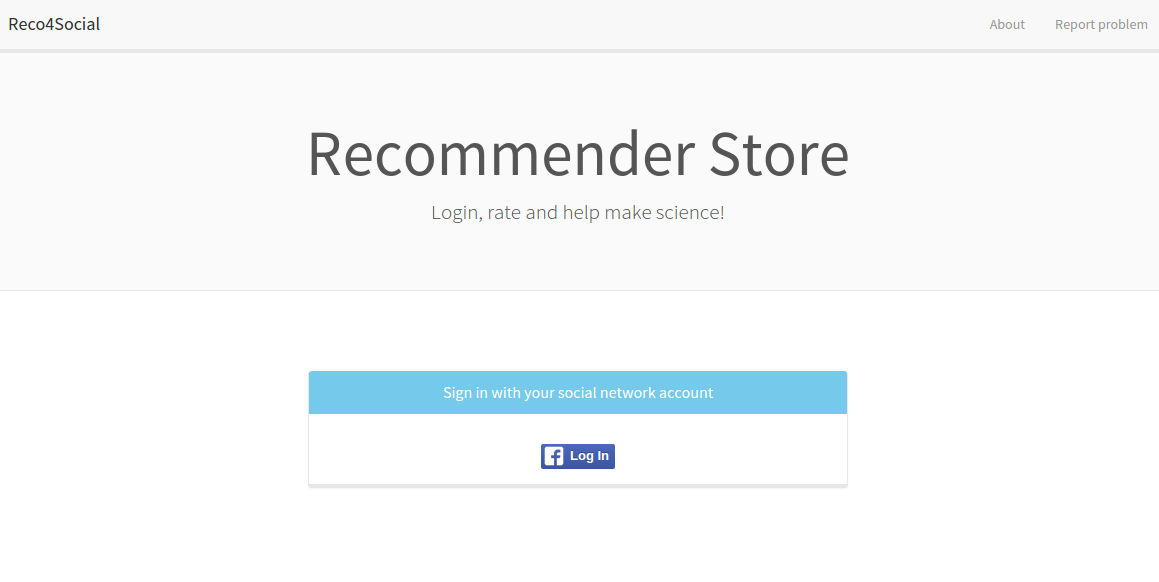
\includegraphics[width=\textwidth]{reco4_login.png} 
\caption[Login page.]{Login page.}
\label{fig.login}
\end{figure}

\begin{figure}[!t]
\centering

\includegraphics[width=7cm]{todo.jpg} 
% width=\textwidth
\caption[Authorizing the Facebook application.]{Authorizing the Facebook application.}
\label{fig.login.fb_app_auth}
\end{figure}

In the background, a Spring component uses the user credentials to query Facebook for additional data. The requested data includes:
\begin{itemize}
\item gender
\item hometown
\item current city
\item political view
\item religion
\item likes - the Facebook pages that the user "likes"
\item friends - only those who have also logged in to my website
\end{itemize}

If during the application authorization process the user edited the sharing options, some or all of the above data may not be accessible.

The received information is processed in the background and stored in the graph database.

\subsubsection{The survey}
\begin{figure}[!t]
\centering
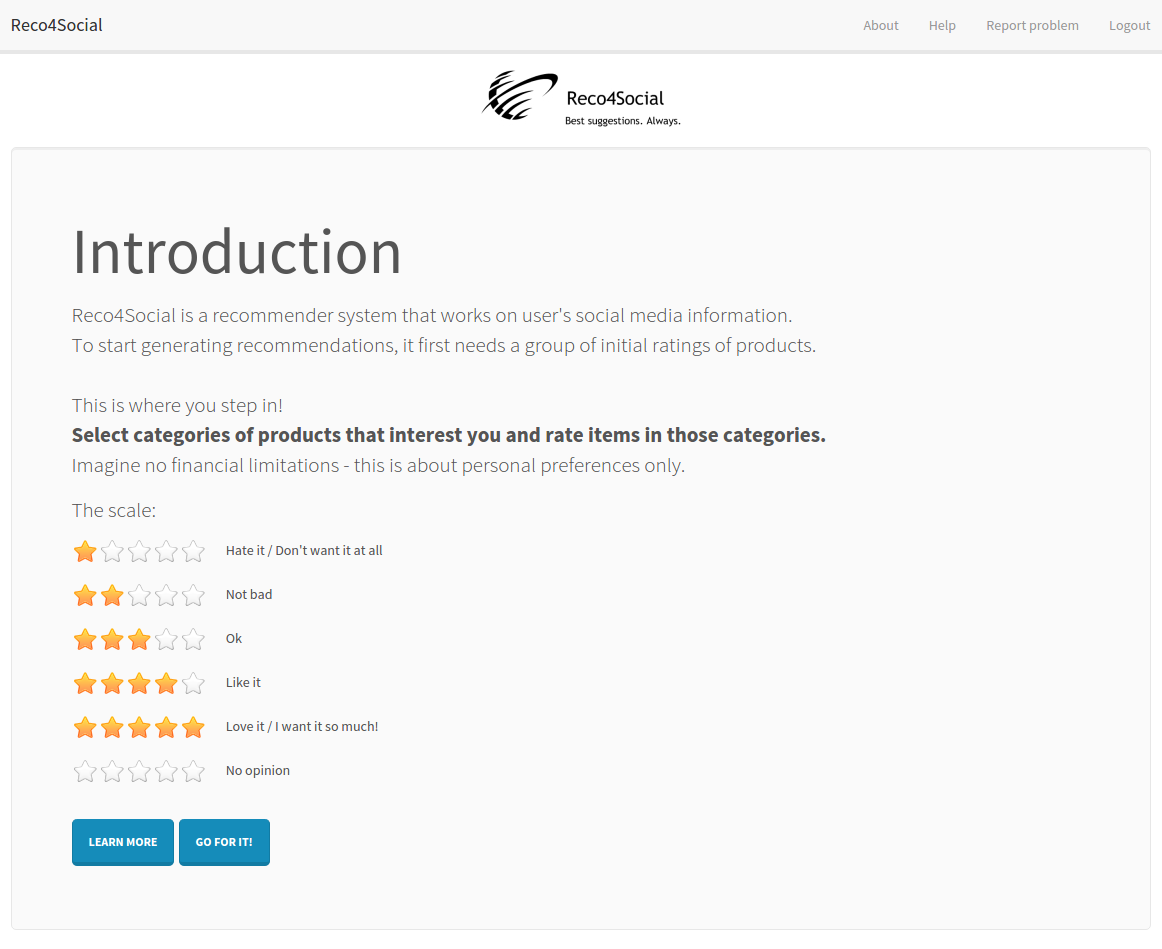
\includegraphics[width=\textwidth]{reco4_survey-intro-1.png} 
\caption[Survey introduction.]{Survey introduction.}
\label{fig.survey.intro-1}
\end{figure}

\begin{figure}[!t]
\centering
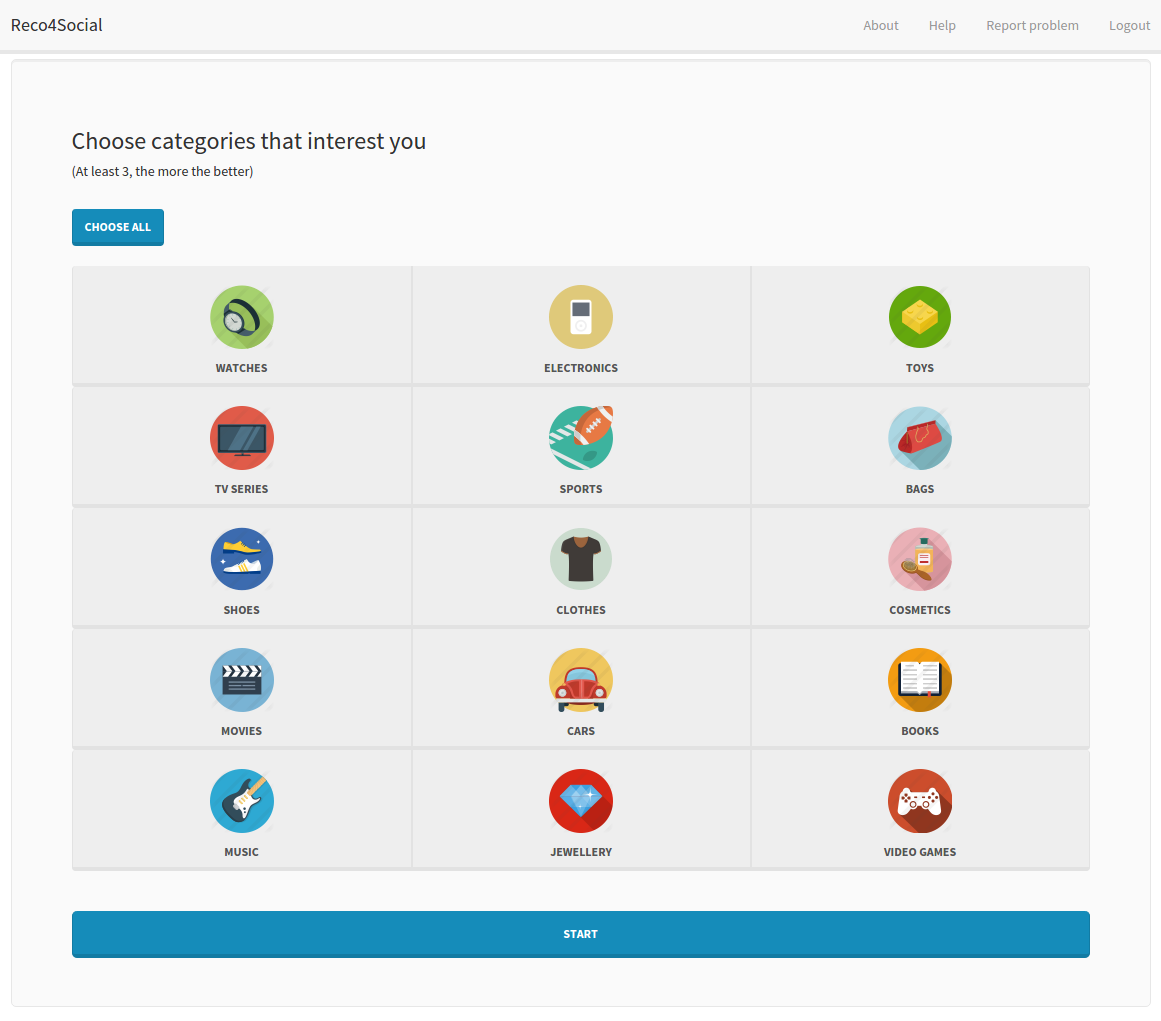
\includegraphics[width=\textwidth]{reco4_survey-intro-2.png} 
\caption[Survey product categories selection.]{Survey product categories selection.}
\label{fig.survey.intro-2}
\end{figure}

\begin{figure}[!t]
\centering

\includegraphics[width=7cm]{todo.jpg} 
% width=\textwidth
\caption[The survey.]{The survey.}
\label{fig.survey}
\end{figure}

\begin{figure}[!t]
\centering

\includegraphics[width=7cm]{todo.jpg} 
% width=\textwidth
\caption[The survey end.]{The survey end.}
\label{fig.survey.end}
\end{figure}

After having successfully logged in, the user is presented with an introduction to the survey, visible in Figure \ref{fig.survey.intro-1}. It explains what the project is about and how to complete the survey, including the description of the rating system.

Users are supposed to choose categories of products that interest them (at least three) and then to rate products in those categories according to their tastes. The rating scale is 1-5, where 1 means "do not like at all" and 5 means "love it". If a user has no opinion about a particular product, they are supposed to leave the rating empty.

For those users that seek additional information about the project, there is the "Learn more" button, which opens a popup window with a more detailed explanation.

Figure \ref{fig.survey.intro-2} shows the categories selection panel, which is located just below the introduction. The users are asked to choose at least three categories, otherwise they are not permitted to proceed. The "Start" button redirects the user to the actual survey.

The survey page (Figure \ref{fig.survey}) presents all products from each category, one at a time. At the top a progress bar informs the user how many categories are left. Each product is contained within a "box", displaying the item's name, picture, price and the rating to be filled. The rating is presented in the form of "stars".

A button at the bottom reloads the page presenting products from the next category. In the case of the last category, it redirects to the survey end page. It is shown in Figure \ref{fig.survey.end} and contains the acknowledgement of the user's contribution to the project.

\subsubsection{The recommender}
[TODO]

\subsection{Implementation}

\subsubsection{Facebook application configuration}
The first step in using the Facebook API is application creation. User data can only be accessed when they grant the appropriate privileges to our application.

The place for managing Facebook applications is the Developers center, available at the URL: \url{https://developers.facebook.com/}.

A new App is created instantaneously, however at first it possesses only the basic permissions for accessing users' data, namely the \url{public_profile}, \url{email} and \url{user_friends} items.

In order to gain permissions for additional information, an approval submission needs to be filled in. Facebook expects detailed explanation, along with screenshots of the website, of how the obtained data will be used. At first my submission was rejected, however the second time, after having stressed that my project is not commercial, but purely academic, the permissions were granted.

In the end my Facebook App has the following permissions that are used in the project:
\begin{itemize}
\item \url{public_profile}
\item \url{user_friends}
\item \url{user_hometown}
\item \url{user_location}
\item \url{user_religion_politics}
\item \url{user_likes}
\end{itemize}

\subsubsection{The login}

\subsubsection{The survey}

\subsubsection{The recommender}

%
\section{User data model in Neo4j}

\subsection{Introduction to Graph Databases}

\subsection{Data model}

\section{Recommendation algorithm}

\chapter{Evaluation}
\section{Evaluation of predictive and classification accuracy}
\section{Evaluation of computation time and resource consumption}
\section{Comparison to non-social recommender systems}

\chapter{Summary and conclusions}
\section{Usability of the project in AMG.net}
\section{Future development perspectives}

% \chapter{Bibliography}

% \chapter{Appendices}

\addcontentsline{toc}{chapter}{Bibliography} 
\begin{thebibliography}{99}
% \bibitem{kacprzyk86}
% Kacprzyk J. (1986) Fuzzy sets in system analysis.  PWN, Warsaw (in Polish).
% \bibitem{kacprzyk99b}
% Kacprzyk J., Strykowski P. (1999) Linguistic Data Summaries for Intelligent Decision Support, Proceedings of EFDAN'99. 4-th European Workshop on Fuzzy Decision Analysis and Recognition Technology for Management, Planning and Optimization, Dortmund, 1999, 3--12.
% \bibitem{kacprzyk01d}
% Kacprzyk J., Yager R. R. (2001) Linguistic summaries of data using fuzzy logic. International Journal of General Systems 30:133--154 
\bibitem{rise_of_social_commerce}
Lora Cecere. \textit{Rise of Social Commerce} [online]. Altimeter [access: 1 May 2015]. Accessible online: \url{http://www.riseofsocialcommerce.com/wp-content/uploads/2010/10/Lora_Cecere-Rise_of_Social_Commerce.pdf}
\bibitem{snrs}
Jianming He, Wesley W. Chu. \textit{A Social Network-Based Recommender System (SNRS)} [online]. Computer Science Department, University of California [access: 25 April 2015]. Accessible online: \url{http://www.cobase.cs.ucla.edu/tech-docs/jmhek/snrs.pdf}
\bibitem{social_login}
Loren McDonald. \textit{Social Login: A Data Capture Game Changer} [online]. Silverpop blog (An IBM Company), 29 November 2011 [access: 28 August 2015]. Accessible online: \url{http://www.silverpop.com/blogs/email-marketing/social-login-data-capture.html}
\bibitem{spring_framework}
\textit{Spring Framework} [online]. Pivotal Software [access: 28 August 2015]. Accessible online: \url{http://projects.spring.io/spring-framework/}
\bibitem{lumen}
\textit{Lumen} [online]. Bootswatch [access: 28 August 2015]. Accessible online: \url{https://bootswatch.com/lumen/}
\bibitem{restfb}
\textit{RestFB} [online]. [access: 28 August 2015]. Accessible online: \url{http://restfb.com/}
\bibitem{neo4j}
\textit{Neo4j} [online]. [access: 28 August 2015]. Accessible online" \url{http://neo4j.com/}

\end{thebibliography}

\addcontentsline{toc}{chapter}{List of figures} 
\listoffigures

\addcontentsline{toc}{chapter}{List of tables} 
\listoftables


\addcontentsline{toc}{chapter}{Appendices} 
\chapter*{Appendices}
\begin{enumerate}
\item Appendix 1
\item Appendix 2
\item Appendix 3
\end{enumerate}

% % %

% \chapter{Dalsze uwagi o edycji i~formatowaniu pracy}
% Pracę w \LaTeX'u najlepiej składać w szablonie {\tt report}, ze względu na jendostronny wydruk (jak w {\tt article}) i możliwość dzielenia pracy na rozdziały, a co za tym idzie, tworzenia spisu treści, spisu tabel, rysunków. 
% \begin{example}
% Przyklad
% \end{example}

% \begin{corollary}
% Wniosek
% \end{corollary}
% \section{Bibliografia i przypisy}
% Spis litertury dołącza się  w \LaTeX'u automatycznie na końcu pracy (zob.
% komenda {\tt begin{thebibliography}}). Informacje o sposobie cytowania zawarte
% są na stronie Bibilioteki Głównej PŁ\\ także udostępnione na
% \underline{\tt http://ics.p.lodz.pl/\textasciitilde aniewiadomski}. \\

% \indent Przykład cytowania --  jak podaje praca \cite{kacprzyk86}, ......,
% jednakże autorzy [2] twierdzą, iż.....\\


% \indent Za każdym razem, kiedy w pracy pojawia się treść na podstawie jakiegoś
% tekstu źródłowego czyjegoś autorstwa, oznaczamy takie miejsce
% przypisem\footnote{Treść przypisu pierwszego}. Przypis zawierać musi  numer
% jakim w spisie literatury, czyli bibliografii, oznaczono tę pracę, np.
% tak\footnote{[3], ss. 3--6 (czyli praca trzecia w spisie literatury,
% wykorzystany fragment znajduje się na stronach od 3. do 6.)}. {\bf
% Wszystkie źródła tekstów, rysunków, danych, wykresów, schematów, kodów i
% informacji wykorzystanych w pracy muszą być zamieszczone w bibliografii.
% Wszystkie pozycje literatury zamieszczone w bibliografii muszą być cytowane w
% treści pracy, na dowód, iż zostały rzeczywiście użyte przy pisaniu pracy.}

% \subsubsection{Źródła elektroniczne}
% Źródła elektroniczne, zwłaszcza internetowe należy cytować z należytą uwagą na
% ich jakość. Nie cytujemy źródeł wątpliwej jakości lub wtórnie przekazujących
% czy też powielających wiedzę zawartą w innych źródłach, np. fora internetowe lub
% wikipedia.\\
% \indent {\bf Wszystkie wykorzystane źródła elektroniczne powinny być przez Autora
% pracy skopiowane \underline{w dniu ich wykorzystania} i
% dołączone np. na CD/DVD do wersji drukowanej pracy.\\
% \indent Odnośniki do źródeł elektronicznych muszą zawierać pełną ścieżkę, np. do
% pliku lub rysunku, a nie jedynie domenowy adres portalu, np.\newline {\tt
% http://serwer.com/temat/podtemat/katalog/plik\_strony.html} (stan na dzień:
% 2009-12-05)\\
% ale nie\\
% {\tt www.portal.pl}.} (!!!!!)

% Niedochowanie tego wymogu może stać się powodem odrzucenia pracy ze wzglę\-dów
% formalnych (,,brak możliwości weryfikacji źródeł wykorzystanych w pracy''). 

% \section{Polskie akapity, cudzysłowy, itp.}
% Akapity stosujemy zawsze z wcięciem, ale bez wiersza odstępu pomiędzy akapitami. 
% Ta forma jest przyjęta dla publikacji polskojęzycznych. {\bf W szczególnych
% przypadkach (także w tym szablonie)} akapit występujący bezpośrednio po tytule
% rozdziału, sekcji, podsekcji itp. NIE JEST WCIĘTY.\\
% \indent Ten akapit JEST WCIĘTY. NIE MA także PUSTEGO WIERSZA pomiędzy tym
% akapitem a poprzednim. \\
% \indent Podobne uwagi dotyczą wszystkich innych elementów formatowania pracy --
% muszą być zgodne ze zwyczajami przyjętymi W JĘZYKU POLSKIM.	Np. cu\-dzysłowy
% wyglądają tak: ,,cudzysłów'', ale nie ''cudzysłów'', albo też `cudzysłów' czy
% ``cudzysłów''. 



% \section{Definicje i wyrażenia matematyczne}
% \begin{definition} \label{def.definicja1}
% Niech $\cal X$ będzie przestrzenią.....
% \end{definition}

% Do definicji odnieść sie można poprzez jej etykietę: jak podano w Def.~\ref{def.definicja1}

% Przykładowe podkreślenie... \underline{tekst podkreślony}, pogrubienie: {\bf
% tekst pogrubiony} oraz wyrożnienie {\em tekst wyróżniony, czyli kursywa}. 
% Dalszy tekst rozdziału
% Dalszy tekst rozdziału
% Dalszy tekst rozdziału
% Dalszy tekst rozdziału
% Dalszy tekst rozdziału
% Dalszy tekst rozdziału
% Dalszy tekst rozdziału
% Dalszy tekst rozdziału
% Dalszy tekst rozdziału a teraz koniec linii... \\
% \indent ... i nowy akapit. Akapity muszą być standardowo wcięte.  


% Przykład wzoru matematycznego numerowanego

% \begin{equation} \label{wzoreinsteina}
% E=m\cdot c^2
% \end{equation}

% {\bf Wszystkie symbole matematyczne występujące w tekście ,,na bieżąco'',
% czyli nieoznaczone numerem równania TAKŻE PISZEMY W TRYBIE MATEMA\-TYCZNYM, CZYLI
% K U R S Y W Ą} : $a=b\cdot c$, ale nie: a= b*c (!!)\\

% \indent Numeracja wzoru -- ZAWSZE w POSTACI (\#.\#\#)
% Jak podaje wzor (\ref{wzoreinsteina}).... (koniec linii). \\
% \indent Wyrażenia matematyczne można też wpisywać w wierszu -- używamy wów\-czas znaku '\$', który rozpoczyna i kończy wyrażenie, np. wg Einsteina $E=m\cdot c^2$...


% \section{Jak wstawiać rysunki? tabele? }
% A teraz pora na rysunek:
% \begin{figure}[!t]
% \centering
% \includegraphics[width=7cm]{1figmftall} 
% \caption{Funkcja przynależności zbioru rozmytego -- Podpis ZAWSZE POD rysunkiem,
% numeracja w postaci \#.\#\#. } (wypada podać źródło, czyli literaturę,
% z której rysunek pochodzi, ewentualnie {\em opracowanie własne}.)
% \label{fig.funkcja.przyn}
% \end{figure}


% \begin{table}[!t]
% \centering
% \caption{Tytuł tabeli ZAWSZE NAD TABELĄ, numeracja w formie \#.\#\#. (wypada podać źródło, czyli literaturę,
% z której tabela pochodzi, ewentualnie {\em opracowanie własne}.)} 

% \label{tabls1}

% {\footnotesize 
% \vspace{5mm}
% \begin{tabular}{c c c c c}
% \hline\noalign{\smallskip}
% {\bf Alg.} & {\bf tytuł kolumny 1} & {\bf tytuł kolumny 1} & {\bf Tytuł kolumny
% 3} & {\bf ....}     \\

% \hline\noalign{\smallskip}
% a & b & c & d & e  \vspace{3mm} \\ 
% \noalign{\smallskip}
%  a & b & c & d & e \\

% \noalign{\smallskip}
% %%%
% \end{tabular}
% }
% \end{table}


% Rysunki i tabele nie powinny przekraczać 0.9 szerokości tekstu i zasadniczo
% powinny występować na górze strony. \\

% \indent Odnosić się do rysunku można poprzez jego etykietę ''label'', np. jak widać na rys. \ref{fig.funkcja.przyn}......

% Jak widać, rysunek nie wypada w dokumencie w tym samym miejscu co w kodzie, choć czasem się tak zdarza. Jeśli potrzebujesz przenieść rysunek, zajrzyj do rozdzialu 2.11. manuala pt. {\em Wstawki}. 

% \section{Listy wypunktowana i numerowana}

% \begin{itemize}
% \item pierwszy element listy wypunktowanej
% \item drugi...
% \item trzeci...
% \end{itemize}


% Nowy akapit z lista numerowaną. 
% \begin{enumerate}
%  \item pierwszy element listy NUMEROWANEJ
%  \item drugi...
%  \item trzeci...
%  \item trzeci...
%  \item trzeci...
%  \end{enumerate}

% \section{Przenoszenie wyrazów}
% Skorzystaj z polecenia {\tt hyphenation}\\ w preambule dokumentu, lub dziel
% wyrazy ,,ręcznie'' czyli właśnie tak jak tu: po\-dzie\-lo\-ne wy\-ra\-zy. 

% \chapter[Technologie i metody użyte...]{Technologie i metody użyte w~części
% badawczej}

% {\em Tytuł tego rozdziału ma dwie wersje: zwykłą, (w kodzie: w nawiasach
% klamrowych), która
% pokazuje sie na stronie rozpoczynającej rozdział, oraz krótką (w kodzie: w nawiasach
% kwadratowych), która pokazuje sie w spisie treści i w nagłówku}

% W rozdziale \ref{fundamental_info} podano podstawy teoretyczne i ogólny zakres
% pracy. W niniejszym rozdziale opisana zostanie technologia XYZ oraz metoda ABC
% użyta w części praktycznej, patrz rozdział~\ref{rozdz.czesc.prakt}. 

% \section{Sprzęt}
% ...................
% \subsection{Element 1}
% .........................
% \subsection{Element 2}
% ......................

% \section{Oprogramowanie}
% ..........................
% \subsection{Serwer baz danych}
% ........................
% \subsection{Środowisko zintegrowane}
% ..........................
% \subsection{Oprogramowanie klienckie}

% \section{Technologie i metodologie programistyczne}
% ..................
% \subsection{Język programowania}
% ......................
% \subsection{Biblioteki}
% .......................
% \subsection{Wzorce projektowe}
% .......................

% \section{Inne, np. narzędzia i metody symulacji, }

% \chapter{Aplikacja/system/projekt "XYZ"} \label{rozdz.czesc.prakt}
% Ta część pracy może być podzielona na więcej rozdziałów, np kiedy autor chce
% w~szczególności podkreślić któryś z etapów projektu. W zależności od tematu i~celów pracy, pewne sekcje można dodać (np. przy projektowaniu sieci, instalacji
% i~konfiguracji serwerów usług sieciowych), inne zaś pominąć.

% \section{Analiza wymagań}
% \subsection{Studium możliwości}
% \subsection{Wymagania funkcjonalne}
% .................
% \subsection{Ograniczenia projektu}

% \section{Projekt}
% \subsection{Projekt warstwy danych}

% \begin{enumerate}
% \item normalizacje baz danych
% \item projekt bazy/baz 
% \item grupy użytkowników i ich prawa dostępu do danych (zależne od implementacji bazy)
% \item ew. diagramy klas warstwy danych
% \end{enumerate}
% \subsection{Projekt warstwy logiki}
% \begin{enumerate}
% \item Diagramy i scenariusze przypadków użycia
% \item Diagramy przepływu danych (lub ich odpowiedniki)
% \item ew. diagramy klas, wzorce projektowe itp.
% \end{enumerate}

% \subsection{Projekt warstwy interfejsu użytkownika}
% \subsubsection{Wybór środowiska i platformy działania}
% \subsubsection{Rodzaj aplikacji (klient-serwer, thick/thin client, aplikacja
% ,,biurkowa'', usługa, klient hybrydowy, itp.}
% \subsubsection{Technologie projektowania i realizacji interfejsu użytkownika,
% np. biblioteki}


% \section{Implementacja: punkty kluczowe}

% \section{Testy i wdrożenie}
% \subsection{Testy wydajności}
% \subsection{Testy regresyjne}
% \subsection{Testy bezpieczeństwa}
% \subsection{Dalsze testy}
% \subsection{Testy...}

% \section{Konserwacja i inżynieria wtórna}
% Jak przebiega eksploatacja systemu/projektu? Jakie wady i zalety ujawniły się po
% np. 2-miesięcznym okresie testowania i użytkowania? \\
% \indent Jak można skorzystać z tej wiedzy praktycznej pod kątem roz\-bu\-do\-wy pracy? Jakie elementy systemu powinny zostać w pierwszej kolejności zmodyfikowane?  

% \chapter{Podsumowanie}
% \section{Dyskusja wyników}
% Dzięki zrealizowaniu pracy poprawie uległa wydajność ....... Ponadto, o ?? \%
% skrócony został czas ........, a koszty osiągnięcia zamierzonego efektu zostały
% zmniejszone z ???pln do ???pln za godzinę/ dzień/ jednostkę sprzętu.........\\
% \indent Które cele pracy udało sie zrealizować? co z tego wynika? Które cele
% pracy pozostały niezrealizowane i dlaczego? 

% \section[Ocena możliwości wdrożenia...]{Ocena możliwości wdrożenia proponowanych
% \newline rozwiązań...}
% ... ich wartość praktyczna, lokalne i globalne możliwości zastosowania, kwestia
% praw autorskich do powstałych produktów, itp. 

% \section{Perspektywy dalszych badań w dziedzinie}
% Jak można kontynuować tę pracę, zwłaszcza pod kątem studiów
% uzupełniających magisterskich i/lub doktoranckich. Co jeszcze powinno być
% zrobione lub ulepszone? Co należy zmienić lub poprawić w pracy z dzisiejszego punktu widzenia?


% \addcontentsline{toc}{chapter}{Bibliografia} 
% \begin{thebibliography}{99}
% % \bibitem{kacprzyk86}
% % Kacprzyk J. (1986) Fuzzy sets in system analysis.  PWN, Warsaw (in Polish).
% % \bibitem{kacprzyk99b}
% % Kacprzyk J., Strykowski P. (1999) Linguistic Data Summaries for Intelligent Decision Support, Proceedings of EFDAN'99. 4-th European Workshop on Fuzzy Decision Analysis and Recognition Technology for Management, Planning and Optimization, Dortmund, 1999, 3--12.
% % \bibitem{kacprzyk01d}
% % Kacprzyk J., Yager R. R. (2001) Linguistic summaries of data using fuzzy logic. International Journal of General Systems 30:133--154 
% \bibitem{rise_of_social_commerce}
% Lora Cecere. \textit{Rise of Social Commerce} [online]. Altimeter [access: 1 May 2015]. Accessible online: \url{http://www.riseofsocialcommerce.com/wp-content/uploads/2010/10/Lora_Cecere-Rise_of_Social_Commerce.pdf}
% \bibitem{snrs}
% Jianming He, Wesley W. Chu. \textit{A Social Network-Based Recommender System (SNRS)} [online]. Computer Science Department, University of California [access: 25 April 2015]. Accessible online: \url{http://www.cobase.cs.ucla.edu/tech-docs/jmhek/snrs.pdf}
% \bibitem{social_login}
% Loren McDonald. \textit{Social Login: A Data Capture Game Changer} [online]. Silverpop blog (An IBM Company), 29 November 2011 [access: 28 August 2015]. Accessible online: \url{http://www.silverpop.com/blogs/email-marketing/social-login-data-capture.html}
% \bibitem{spring_framework}
% \textit{Spring Framework} [online]. Pivotal Software [access: 28 August 2015]. Accessible online: \url{http://projects.spring.io/spring-framework/}

% \end{thebibliography}

% \addcontentsline{toc}{chapter}{Spis rysunków} 
% \listoffigures

% \addcontentsline{toc}{chapter}{Spis tabel} 
% \listoftables


% \addcontentsline{toc}{chapter}{Załączniki} 
% \chapter*{Załączniki}
% \begin{enumerate}
% \item Załącznik nr 1
% \item Załącznik nr 2
% \item Załącznik nr 3
% \end{enumerate}


\end{document}

